\chapter{Déploiement du Système d'information}
%\markboth{Chapitre 3 }{Déploiement du Système d'information} %pour afficher l'entete
 %\addcontentsline{toc}{chapter}{Chapitre 3 : Déploiement du Système d'information}


\section{Introduction}


Le déploiement du système d'information est une étape cruciale pour toute entreprise moderne. Afin de répondre aux besoins spécifiques de Zeta Engineering, nous avons identifié les éléments essentiels à intégrer dans notre système d'information, tels que le protocole DHCP, la plateforme Asterisk, ainsi que les modules ERP et CRM, etc. Cette sélection nous permettra de mettre en place une base solide pour notre système d'information. Par la suite, l'équipe informatique se concentrera sur l'amélioration progressive du SI, en effectuant des ajustements et des optimisations. \\


Dans ce chapitre, nous détaillerons les différentes étapes du déploiement de ces systèmes d'information, en commençant par l'installation et la configuration des serveurs nécessaires à leur fonctionnement. Nous expliquerons également les choix techniques que nous avons effectués pour répondre aux exigences de l'entreprise et assurer une infrastructure robuste et sécurisée. \cite{opg} \\


\newpage


\section{Les solutions choisies}

Le tableau suivant montre les solutions essentiel choisis pour intégrer a notre entreprise système d'informations 

\begin{table}[H]
\begin{center}
\begin{tabular}{|c{3cm}|c{3cm}|c{8cm}|}
\hline
OS Serveur & Ubuntu Server & Plateforme de système d'exploitation robuste et stable basée sur Linux, offrant un environnement fiable et sécurisé pour les serveurs. \\
\hline
Virtualisation & KVM & Permettre l'exécution de systèmes virtuels sur différents systèmes d'exploitation en simulant du matériel standardisé. \\
\hline
DHCP & ISC DHCP & Offre des fonctionnalités avancées pour la configuration et la gestion des adresses IP. ISC DHCP est souvent utilisé comme serveur DHCP dans les environnements Linux, notamment sur la distribution Ubuntu. \\
\hline
ERP/CRM & Odoo & Plateforme intégrée de gestion d'entreprise qui offre des fonctionnalités pour la gestion des ressources, des ventes, des finances, des ressources humaines et bien plus encore. \\
\hline
Voip / Téléphonie & Asterisk & Gérer les appels téléphoniques, y compris la gestion des lignes et d'autres fonctionnalités avancées. Il prend en charge différents protocoles de communication, tels que SIP et RTP, permettant ainsi la mise en place de communications vocales à travers le réseau IP. \\
\hline
Gestion de parc et d'inventaires & GLPI & Suivre et gérer les actifs matériels et logiciels d'une organisation, y compris les utilisateurs, les ordinateurs, les périphériques et les licences logicielles. \\
\hline
Gestion des identités et contrôle d'accès & OpenLDAP & Gérer les utilisateurs, les ordinateurs et les groupes au sein d'un réseau. Fournir des fonctionnalités d'authentification, de contrôle d'accès et de gestion des politiques de sécurité. \\
\hline
\end{tabular}
\caption{Les Solutions Choisis pour le Système d'information}
\label{1}
\end{center}
\end{table}


\section{Déploiement de solutions choisies}

\begin{figure}[H]
 \centering
    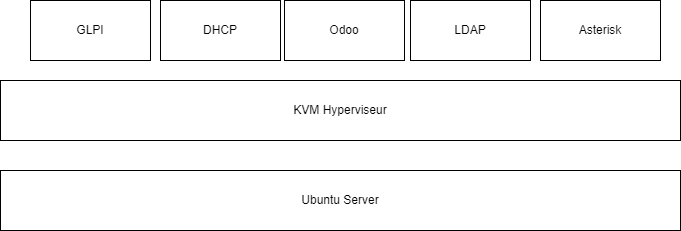
\includegraphics[width=15cm]{Images/diagsi.png}
    \caption{Diagramme du Système d'information}
    \label{fig:diagramme-SI}
\end{figure}



\subsection{OS Serveur}
Nous avons choisi Ubuntu Server 22.04 pour son excellente performance, sa stabilité et sa compatibilité avec un large éventail de logiciels et de technologies. Ubuntu Server est une distribution Linux légère spécialement conçue pour les serveurs, ce qui en fait un choix idéal pour notre environnement. \\


Ubuntu Server 22.04 est la dernière version de la distribution serveur d'Ubuntu, basée sur le système d'exploitation Linux. Elle offre une multitude de fonctionnalités et d'améliorations par rapport aux versions précédentes, notamment : \\

\begin{itemize}
  
\item Performances améliorées : Ubuntu Server 22.04 est optimisé pour fournir des performances élevées, permettant ainsi de gérer efficacement les charges de travail les plus exigeantes.

\item Sécurité renforcée : La distribution intègre des fonctionnalités de sécurité avancées, telles que la prise en charge du chiffrement des données, les mises à jour automatiques et la gestion des certificats, afin de garantir la confidentialité et l'intégrité des données.

\item Support à long terme : Ubuntu Server 22.04 bénéficie d'un support à long terme (LTS) de cinq ans, ce qui signifie que des mises à jour de sécurité et des correctifs seront disponibles pendant une période prolongée, assurant ainsi la stabilité et la fiabilité du système.

\item Écosystème riche : Ubuntu Server est soutenu par une vaste communauté d'utilisateurs et de développeurs, ce qui garantit un support et une documentation abondants, ainsi qu'un large éventail de logiciels et d'outils disponibles pour répondre aux besoins spécifiques du serveur.
\end{itemize}



Voici notre connexion à notre serveur Ubuntu 22.04 grâce à Putty en figure \ref{fig:putty-connection} : \\

\begin{figure}[H]
 \centering
    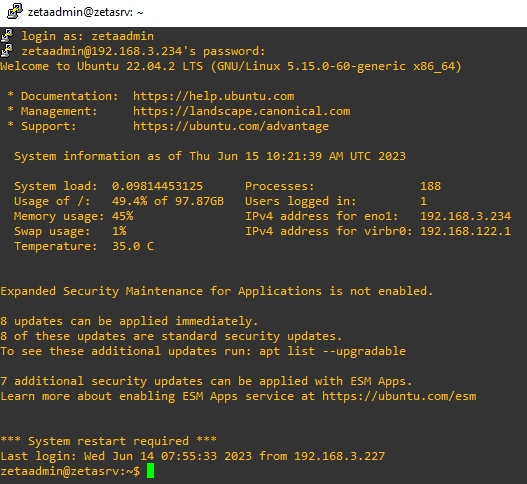
\includegraphics[width=15cm]{Images/zetaserver.png}
    \caption{Connexion à Ubuntu Server 22.04 via Putty}
    \label{fig:putty-connection}
\end{figure}

Ci-dessous \ref{fig:neofetch-result}, vous pouvez voir le résultat de la commande "neofetch" exécutée sur notre serveur Ubuntu : \\

\begin{figure}[H]
 \centering
    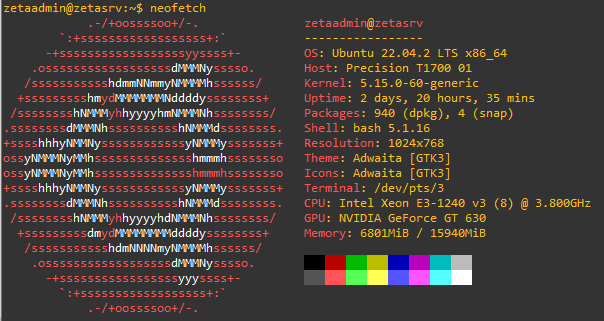
\includegraphics[width=15cm]{Images/neofetchzetasrv.png}
    \caption{Résultat de la commande "neofetch" sur Ubuntu Server 22.04}
    \label{fig:neofetch-result}
\end{figure}



\subsection{Visualisation}
Nous avons choisi KVM (Kernel-based Virtual Machine) pour sa performance et sa compatibilité avec Ubuntu Server, afin d'héberger nos machines virtuelles (VM). KVM est une solution de virtualisation open source qui permet d'exécuter des systèmes virtuels sur un serveur physique. \\

Avant d'installer KVM, nous avons effectué les vérifications suivantes pour nous assurer de la compatibilité matérielle : \\

1. Nous avons exécuté la commande `egrep -c '(vmx|svm)' /proc/cpuinfo` pour vérifier la présence des instructions de virtualisation matérielles (VT-x pour Intel ou AMD-V pour AMD) sur le processeur. Un résultat supérieur à zéro indique que le processeur prend en charge la virtualisation matérielle. \\

2. Nous avons utilisé la commande `kvm-ok` pour vérifier si les modules de virtualisation étaient chargés correctement dans le système et si la virtualisation était supportée. \\

Une fois ces vérifications réussies, nous avons procédé à l'installation des packages nécessaires en exécutant la commande suivante : `sudo apt install -y qemu-kvm virt-manager libvirt-daemon-system virtinst libvirt-clients bridge-utils` v

Ci-dessous, vous pouvez voir les captures d'écran illustrant les étapes d'installation de KVM et de vérification de l'état du service libvirtd dans les figures  \ref{fig:kvm-installation} et \ref{fig:libvirtd-status}  : \\

\begin{figure}[H]
 \centering
    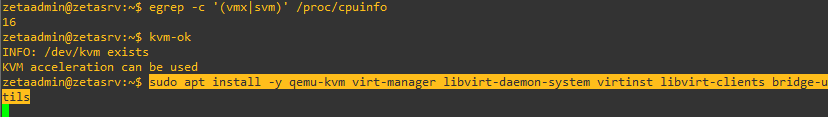
\includegraphics[width=15cm]{Images/installkvm1.png}
    \caption{Installation des packages KVM}
    \label{fig:kvm-installation}
\end{figure}

\begin{figure}[H]
 \centering
    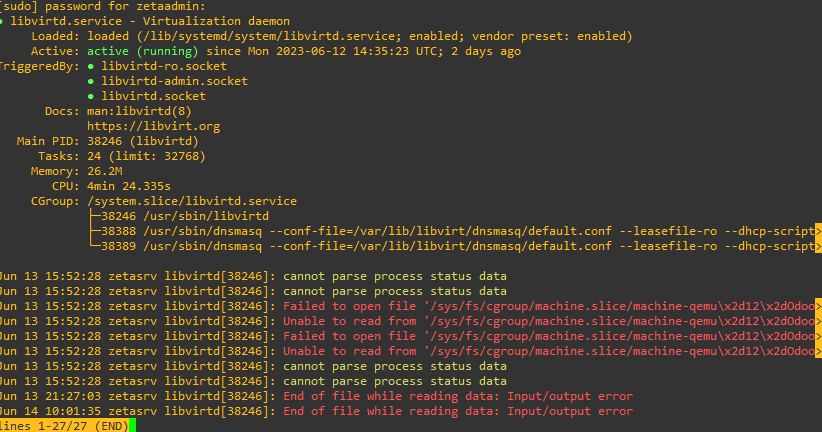
\includegraphics[width=15cm]{Images/installkvm2.png}
    \caption{Vérification de l'état du service libvirtd}
    \label{fig:libvirtd-status}
\end{figure}

Enfin, grâce à l'utilisation de Xming et de Putty, nous pouvons accéder au gestionnaire graphique Virt-Manager à distance depuis notre utilisateur Windows. Cela nous permet de configurer nos machines virtuelles de manière conviviale. \\

\begin{figure}[H]
 \centering
    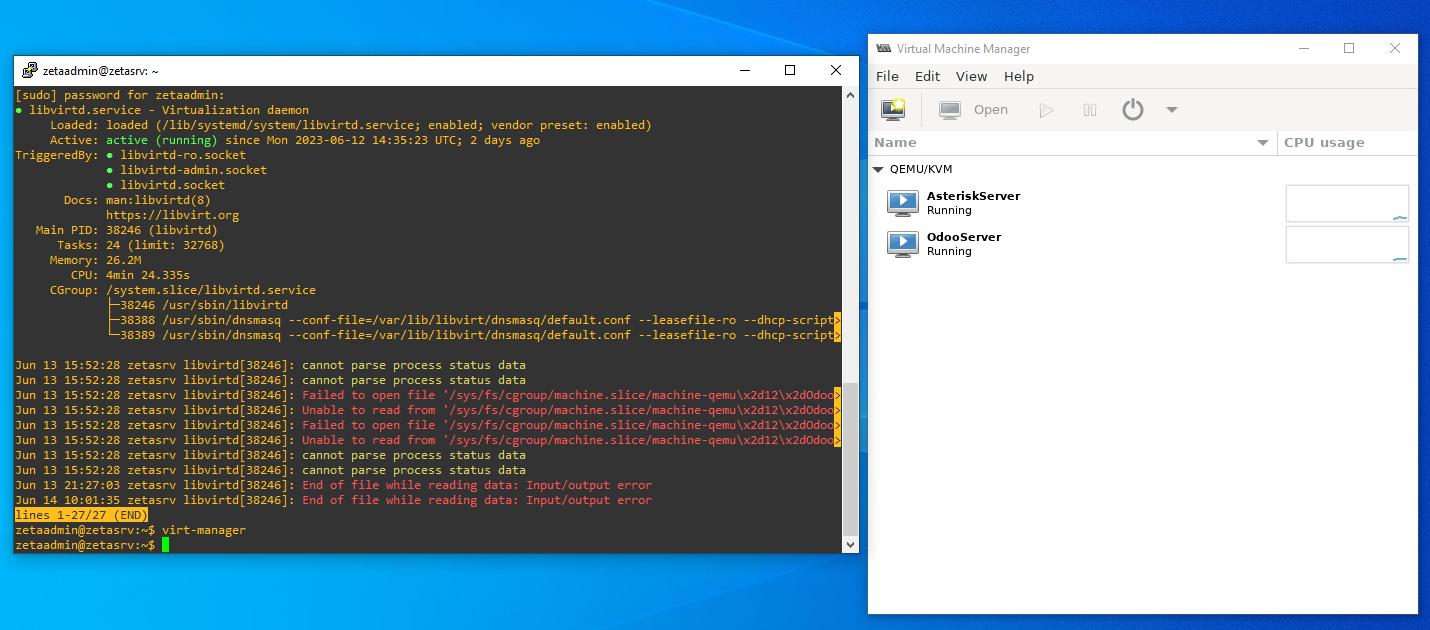
\includegraphics[width=15cm]{Images/resultvirtmanager.png}
    \caption{Accès à Virt-Manager via Xming et Putty}
    \label{fig:virt-manager-access}
\end{figure}

Ainsi, nous pouvons gérer et administrer nos VMs de manière efficace en utilisant Virt-Manager et KVM sur notre serveur Ubuntu comme le montre \ref{fig:virt-manager-access}. \\


\subsection{DHCP}

Pour mettre en place et configurer un serveur DHCP sur une machine virtuelle Linux, nous avons suivi les étapes suivantes : \\

Tout d'abord, nous avons effectué une mise à jour du système Linux en exécutant la commande "apt-get update" dans la figure \ref{fig:update-linux} : \\

\begin{figure}[H]
 \centering
    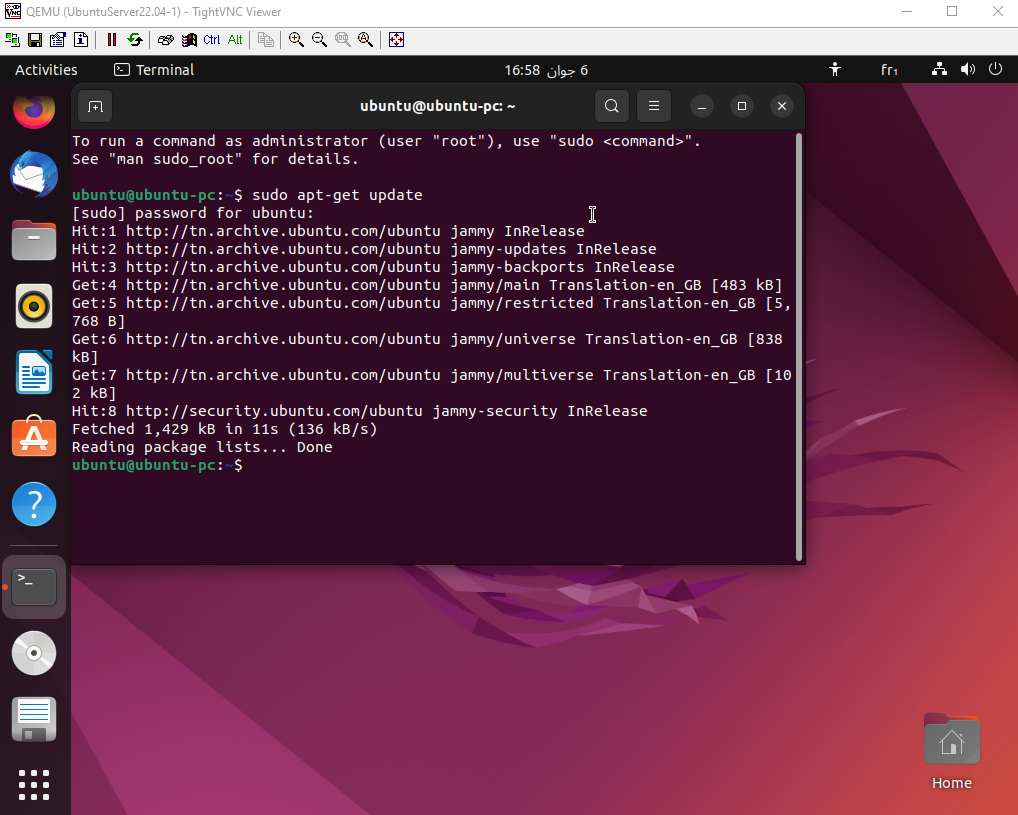
\includegraphics[width=15cm]{Images/dhcp1.png}
    \caption{Mise à jour du système Linux}
    \label{fig:update-linux}
\end{figure}

Ensuite, nous avons redémarré le service isc-dhcp pour appliquer les modifications \ref{fig:restart-isc-dhcp}: \\

\begin{figure}[H]
 \centering
    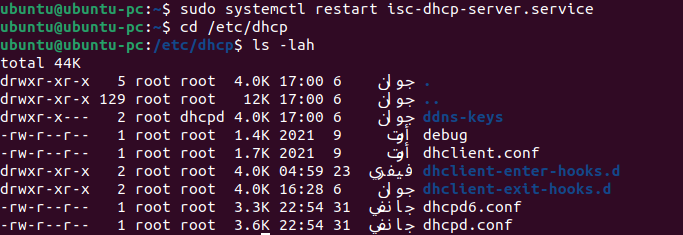
\includegraphics[width=15cm]{Images/dhcp2.png}
    \caption{Redémarrage du service isc-dhcp}
    \label{fig:restart-isc-dhcp}
\end{figure}

Nous avons ensuite procédé à la configuration du fichier dhcpd.conf à l'aide de l'éditeur de texte gedit \ref{fig:dhcpd-conf-configuration} : \\

\begin{figure}[H]
 \centering
    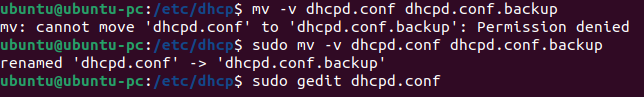
\includegraphics[width=15cm]{Images/dhcp3.png}
    \caption{Configuration du fichier dhcpd.conf}
    \label{fig:dhcpd-conf-configuration}
\end{figure}

Voici un exemple de fichier de configuration dhcpd.conf : \\

\begin{figure}[H]
 \centering
    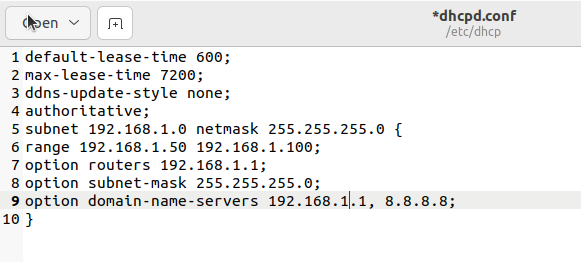
\includegraphics[width=15cm]{Images/dhcp4.png}
    \caption{Exemple de fichier de configuration dhcpd.conf}
    \label{fig:dhcpd-conf-example}
\end{figure}

Enfin, nous avons vérifié que le serveur DHCP ISC était en cours d'exécution en utilisant la commande systemctl status isc-dhcp-server.service : \\

\begin{figure}[H]
 \centering
    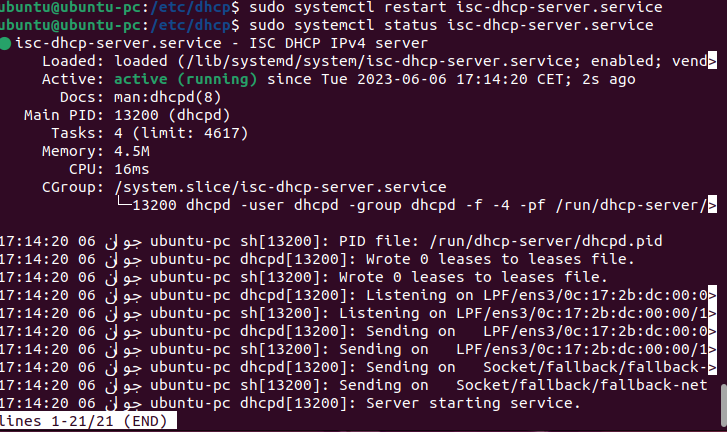
\includegraphics[width=15cm]{Images/dhcp5.png}
    \caption{État du service ISC DHCP}
    \label{fig:isc-dhcp-service-status}
\end{figure}

Ainsi, nous avons réussi à mettre en place et configurer un serveur DHCP sur notre machine virtuelle Linux. Cela nous permettra de fournir automatiquement des adresses IP et d'autres informations de configuration réseau aux clients DHCP de notre réseau. \\



\subsection{VoIP/Téléphonie}

Étant donné que notre entreprise dispose d'une équipe de centre d'appels, il est essentiel d'avoir une solution de téléphonie centralisée comme Asterisk sur notre serveur. Asterisk est un logiciel de téléphonie open source qui permet de gérer les appels téléphoniques, les files d'attente, les routages, etc. Nous avons procédé à la configuration et à l'installation d'Asterisk selon les étapes suivantes : \\

Voici notre installation d'Asterisk sur notre machine virtuelle Ubuntu : \\

\begin{figure}[H]
 \centering
    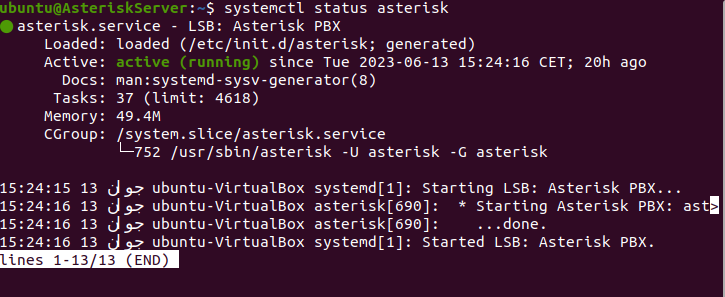
\includegraphics[width=15cm]{Images/AsteriskServer1.png}
    \caption{Installation d'Asterisk sur Ubuntu}
    \label{fig:asterisk-server1}
\end{figure}

Nous avons confirmé le bon fonctionnement d'Asterisk en utilisant le logiciel Zoiper : \\

\begin{figure}[H]
 \centering
    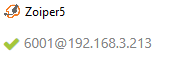
\includegraphics[width=10cm]{Images/AsteriskServer2.png}
    \caption{Confirmation du fonctionnement d'Asterisk avec Zoiper}
    \label{fig:asterisk-server2}
\end{figure}

Veuillez noter que vous pouvez copier le code directement à partir d'ici pour reproduire les figures dans votre propre documentation. \\



\subsection{ERP/CRM}

Odoo est une suite logicielle open-source complète qui propose des modules de gestion d'entreprise, y compris des fonctionnalités ERP (Enterprise Resource Planning) et CRM (Customer Relationship Management).  \\

Odoo offre une large gamme de fonctionnalités et de modules couvrant différents aspects de la gestion d'entreprise, tels que la comptabilité, la gestion des ventes, la gestion des stocks, la gestion des ressources humaines, le marketing, etc. Les modules ERP d'Odoo permettent de gérer efficacement les opérations et les processus internes de l'entreprise, tandis que les modules CRM offrent des outils pour gérer les relations avec les clients et optimiser les activités de vente et de marketing. \\

Le choix d'Odoo en tant que solution ERP/CRM s'explique par plusieurs raisons. Tout d'abord, Odoo est un logiciel open-source, ce qui signifie qu'il est librement accessible et modifiable, offrant ainsi une flexibilité et une personnalisation accrues. De plus, Odoo dispose d'une communauté active qui contribue au développement et à l'amélioration continue du logiciel, ce qui garantit une évolution constante et des mises à jour régulières. \\

Voici un aperçu de notre installation d'Odoo sur notre machine virtuelle Ubuntu : \\

\begin{figure}[H]
 \centering
    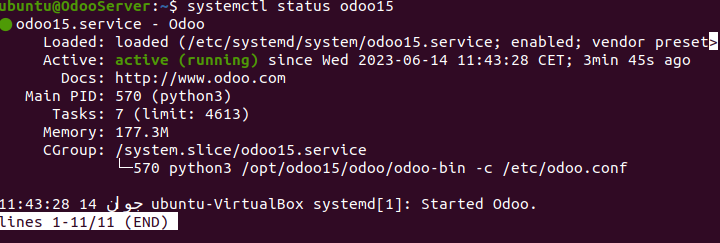
\includegraphics[width=15cm]{Images/OdooServer1.png}
    \caption{Installation d'Odoo sur Ubuntu}
    \label{fig:odoo-installation}
\end{figure}

Et voici la confirmation du bon fonctionnement d'Odoo avec le tableau de bord accessible depuis notre navigateur, où les modules CRM sont installés : \\

\begin{figure}[H]
 \centering
    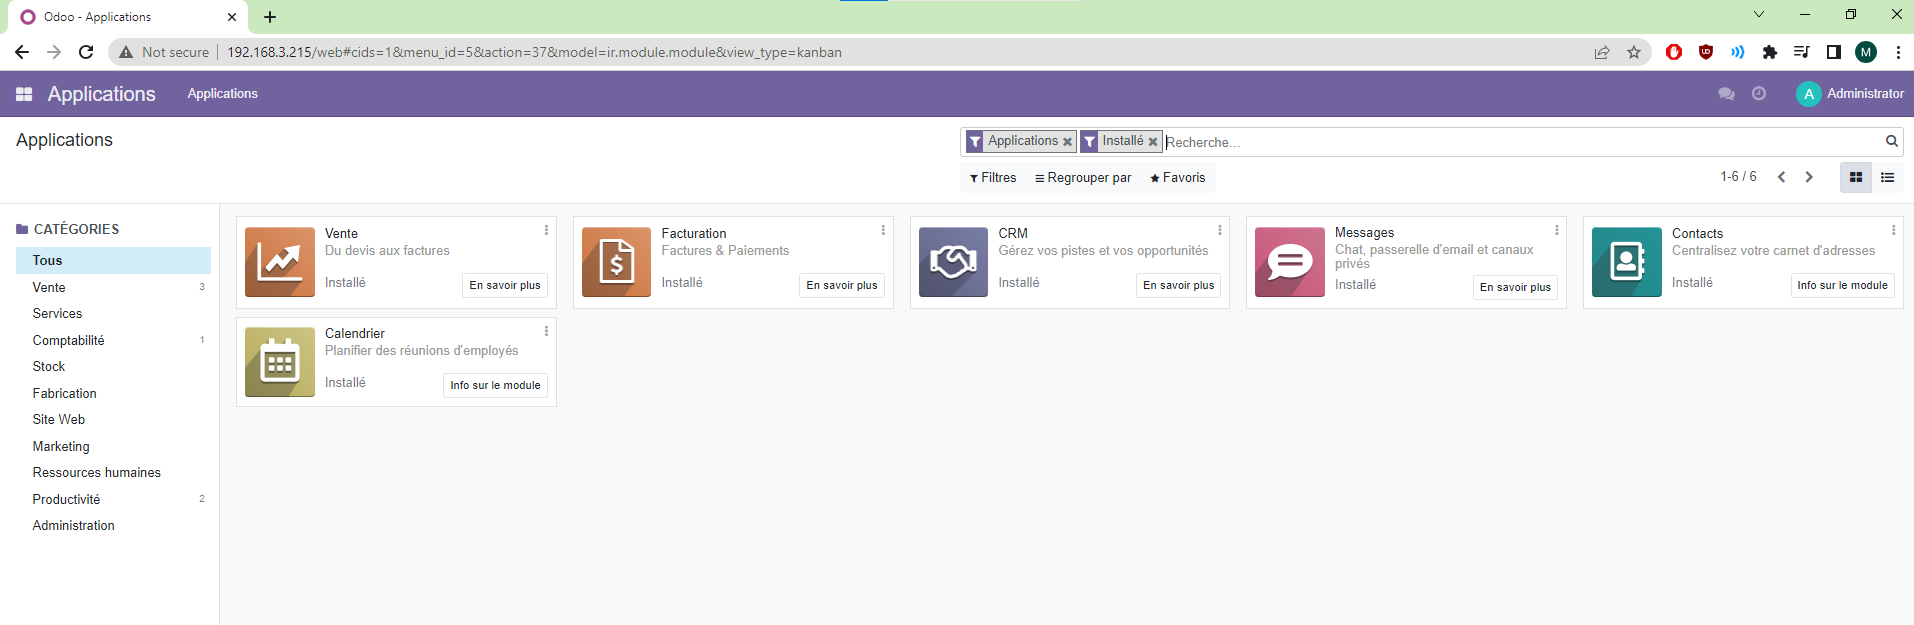
\includegraphics[width=15cm]{Images/OdooServer2.png}
    \caption{Tableau de bord d'Odoo avec les modules CRM installés}
    \label{fig:odoo-dashboard}
\end{figure}

Grâce à Odoo, nous pourrons gérer efficacement nos processus d'entreprise, améliorer nos relations avec les clients et optimiser nos activités de vente et de marketing. La flexibilité, la personnalisation et la communauté active d'Odoo en font une solution ERP/CRM puissante et adaptée à nos besoins. \\



\subsection{GLPI}
GLPI (Gestionnaire Libre de Parc Informatique) est une plateforme open-source largement utilisée pour la gestion des services informatiques et des actifs informatiques. L'un des plugins les plus populaires de GLPI est FusionInventory, qui permet la collecte automatisée des informations sur le matériel et les logiciels du parc informatique. \\

FusionInventory s'intègre parfaitement à GLPI, offrant ainsi une solution complète pour la gestion centralisée des équipements informatiques. Les informations collectées par FusionInventory, telles que les détails matériels, les logiciels installés et les configurations, sont automatiquement importées dans la base de données de GLPI. \\

Cette intégration permet d'avoir une vue d'ensemble complète et à jour du parc informatique de l'entreprise dans le tableau de bord de GLPI. Les responsables informatiques peuvent ainsi avoir une vision claire de tous les équipements, leur localisation, leur état, les utilisateurs associés, etc. \\

Voici un aperçu du tableau de bord de GLPI, où toutes les informations sur les équipements peuvent être consultées et gérées efficacement : \\

\begin{figure}[H]
\centering
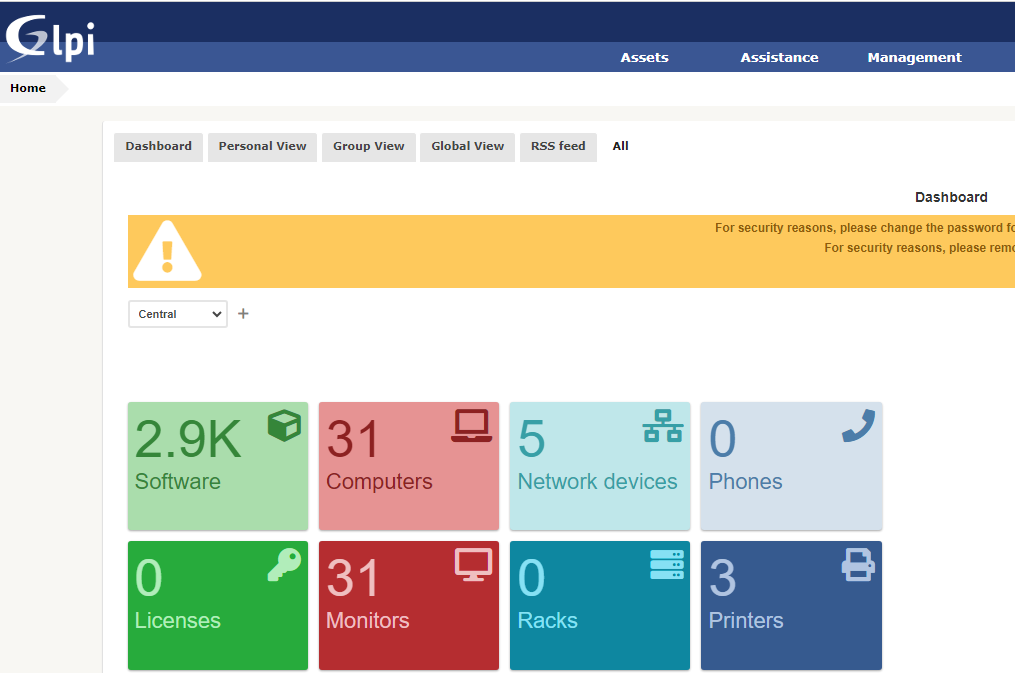
\includegraphics[width=15cm]{Images/GLPI.png}
\caption{Tableau de bord de GLPI}
\label{fig:glpi-dashboard}
\end{figure}

Grâce à GLPI et FusionInventory, les avantages suivants sont obtenus : \\

1. Gestion centralisée des actifs : Tous les équipements, qu'il s'agisse de postes de travail, de serveurs, d'imprimantes ou de périphériques, sont regroupés dans une seule interface. Cela facilite la recherche, la gestion et la maintenance de l'ensemble du parc informatique. \\

2. Automatisation de l'inventaire : Les informations sur le matériel et les logiciels sont collectées automatiquement, réduisant ainsi les erreurs et les efforts manuels. Cela permet d'avoir une base de données à jour et précise de tous les équipements. \\

3. Suivi des incidents et des problèmes : Avec GLPI, il est possible de lier les équipements aux tickets d'assistance, facilitant ainsi la résolution des incidents et le suivi des problèmes techniques. \\

4. Gestion des contrats et des licences : GLPI permet de gérer les contrats de maintenance, les licences logicielles et les garanties associées aux équipements du parc informatique. Cela facilite la gestion des renouvellements, des échéances et des coûts associés. \\

En résumé, l'intégration de FusionInventory avec GLPI offre une solution complète pour la gestion des actifs informatiques et des services informatiques. Elle permet une meilleure visibilité du parc informatique, une automatisation de l'inventaire, une gestion efficace des incidents et des problèmes, ainsi qu'une gestion simplifiée des contrats et des licences. \\

\subsection{openLDAP}

OpenLDAP, un logiciel open-source, est utilisé dans notre système SI pour la gestion des identités et des accès des utilisateurs. Il fournit un serveur d'annuaire LDAP (Lightweight Directory Access Protocol) permettant d'accéder et de gérer les informations de manière centralisée. LDAP est un protocole de communication utilisé pour cette gestion. \\

OpenLDAP offre une gamme de fonctionnalités pour la gestion des utilisateurs, des groupes et des autorisations. Cela facilite l'administration des comptes utilisateurs, la mise en place de politiques de sécurité et la gestion des droits d'accès aux ressources informatiques. En intégrant openLDAP à notre système SI, nous pourrons gérer efficacement les identités et les accès des utilisateurs. \\

Le tableau de bord de phpLDAPAdmin, une interface graphique pour la gestion de l'annuaire LDAP, est présenté ci-dessous. Cependant, il n'a pas encore été configuré et distribué sur tous les postes clients. \\

\begin{figure}[H]
\centering
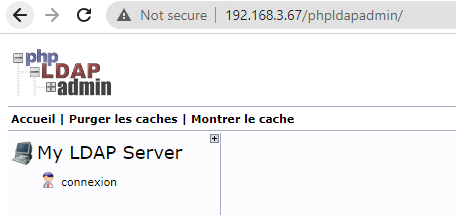
\includegraphics[width=15cm]{Images/ldapdashboard.png}
\caption{Tableau de bord de phpLDAPAdmin}
\label{fig:ldap-dashboard}
\end{figure}

OpenLDAP est reconnu pour ses performances, sa fiabilité et sa flexibilité. Il peut être intégré à d'autres systèmes d'authentification, tels que Kerberos, pour renforcer la sécurité des accès. Sa compatibilité avec de nombreux systèmes et applications facilite son déploiement dans des environnements hétérogènes. En choisissant openLDAP comme solution de gestion des identités et des accès, nous bénéficions d'un système solide et éprouvé pour centraliser et gérer les informations des utilisateurs, renforçant ainsi la sécurité de notre système SI.\\


\newpage

\section{Conclusion}

Le déploiement du système d'information de Zeta Engineering a été réalisé en suivant un processus structuré et en utilisant des solutions techniques adaptées. Nous avons sélectionné avec soin les différents éléments de notre système d'information, tels que le pare-feu pfSense, le système d'exploitation Ubuntu Server, la virtualisation KVM, le serveur DHCP ISC DHCP, le CRM/ERP Odoo, la plateforme de téléphonie Asterisk, ainsi que les outils de gestion des inventaires GLPI et FusionInventory et de gestion des identités OpenLDAP. \\

L'installation et la configuration de ces solutions ont été effectuées en suivant des étapes précises. Nous avons installé pfSense pour assurer la sécurité de notre réseau en contrôlant le trafic entrant et sortant. Ubuntu Server 22.04 a été choisi comme système d'exploitation serveur en raison de sa performance, de sa stabilité et de sa compatibilité avec de nombreux logiciels. La virtualisation KVM a été mise en place pour héberger nos machines virtuelles, tandis que le serveur DHCP ISC DHCP a été configuré pour la gestion des adresses IP. Odoo a été utilisé comme plateforme intégrée de gestion d'entreprise, et Asterisk a été déployé pour la gestion des appels téléphoniques. \\

Ce déploiement a permis à Zeta Engineering de mettre en place une infrastructure solide et sécurisée pour son système d'information. Les choix techniques effectués garantissent une performance élevée, une stabilité et une compatibilité avec les besoins de l'entreprise. L'équipe informatique pourra désormais se concentrer sur l'amélioration progressive du système d'information, en effectuant des ajustements et des optimisations pour répondre aux besoins évolutifs de l'entreprise. \\

En conclusion, le déploiement du système d'information de Zeta Engineering constitue une étape essentielle pour assurer le bon fonctionnement et la performance de l'entreprise. Les solutions techniques choisies offrent une base solide et sécurisée, permettant à l'entreprise de poursuivre ses activités de manière efficace et fiable. \\
